% -*- latex -*-

\subsubsection{\stid{4.13} ECP/VTK-m}

\paragraph{Overview}
The ECP/VTK-m project is providing the core capabilities to perform scientific visualization on Exascale architectures.
The ECP/VTK-m project fills the critical feature gap of performing visualization and analysis on processors like graphics-based processors and many integrated core.
The results of this project will be delivered in tools like ParaView, VisIt, and Ascent as well as in stand-alone form.
Moreover, these projects are depending on this ECP effort to be able to make effective use of ECP architectures.

One of the biggest recent changes in high-performance computing is the increasing use of accelerators.
Accelerators contain processing cores that independently are inferior to a core in a typical CPU, but these cores are replicated and grouped such that their aggregate execution provides a very high computation rate at a much lower power.

Current and future CPU processors also require much more explicit parallelism.
Each successive version of the hardware packs more cores into each processor, and technologies like hyper threading and vector operations require even more parallel processing to leverage each core's full potential.

VTK-m is a toolkit of scientific visualization algorithms for emerging processor architectures.
VTK-m supports the fine-grained concurrency for data analysis and visualization algorithms required to drive extreme scale computing by providing abstract models for data and execution that can be applied to a variety of algorithms across many different processor architectures.

The ECP/VTK-m project is building up the VTK-m codebase with the necessary visualization algorithm implementations that run across the varied hardware platforms to be leveraged at the Exascale.
We will be working with other ECP projects, such as ALPINE, to integrate the new VTK-m code into production software to enable visualization on our HPC systems.

\paragraph{Key  Challenges}
The scientific visualization research community has been building scalable HPC algorithms for over 15 years, and today there are multiple production tools that provide excellent scalability.
However, our current visualization tools are based on a message-passing programming model.
More to the point, they rely on a coarse decomposition with ghost regions to isolate parallel execution \cite{Ahrens2001,Childs2010}.
However, this decomposition works best when each processing element has on the order of a hundred thousand to a million data cells \cite{ParaViewTutorial} and is known to break down as we approach the level of concurrency needed on modern accelerators \cite{Moreland2012:Ultravis,Moreland2013:UltraVis}.

DOE has made significant investments in HPC visualization capabilities.
For us to feasibly update this software for the upcoming Exascale machines, we need to be selective on what needs to be updated, and we need to maximize the code we can continue to use.
Regardless, there is a significant amount of software to be engineered and implemented, so we need to extend our development resources by simplifying algorithm implementation and providing performance portability across current and future devices.


\paragraph{Solution Strategy}
The ECP/VTK-m project leverages VTK-m \cite{Moreland2016:VTKm} to overcome these key challenges.
VTK-m has a software framework that provides the following critical features.

\begin{enumerate}
\item \textbf{Visualization building blocks:}
  VTK-m contains the common data structures and operations required for scientific visualization.
  This base framework simplifies the development of visualization algorithms \cite{VTKmUsersGuide}.
\item \textbf{Device portability:}
  VTK-m uses the notion of an abstract device adapter, which allows algorithms written once in VTK-m to run well on many computing architectures.
  The device adapter is constructed from a small but versatile set of data parallel primitives, which can be optimized for each platform \cite{Blelloch1990}.
  It has been shown that this approach not only simplifies parallel implementations, but also allows them to work well across many platforms \cite{Lo2012,Larsen2015,Moreland2015}.
\item \textbf{Flexible integration:}
  VTK-m is designed to integrate well with other software.
  This is achieved with flexible data models to capture the structure of applications' data \cite{Meredith2012} and array wrappers that can adapt to target memory layouts \cite{Moreland2012:PDAC}.
\end{enumerate}

Even with these features provided by VTK-m, we have a lot of work ahead of us to be ready for Exascale.
Our approach is to incrementally add features to VTK-m and expose them in tools like ParaView and VisIt.


\begin{figure}[t]
  \centering
  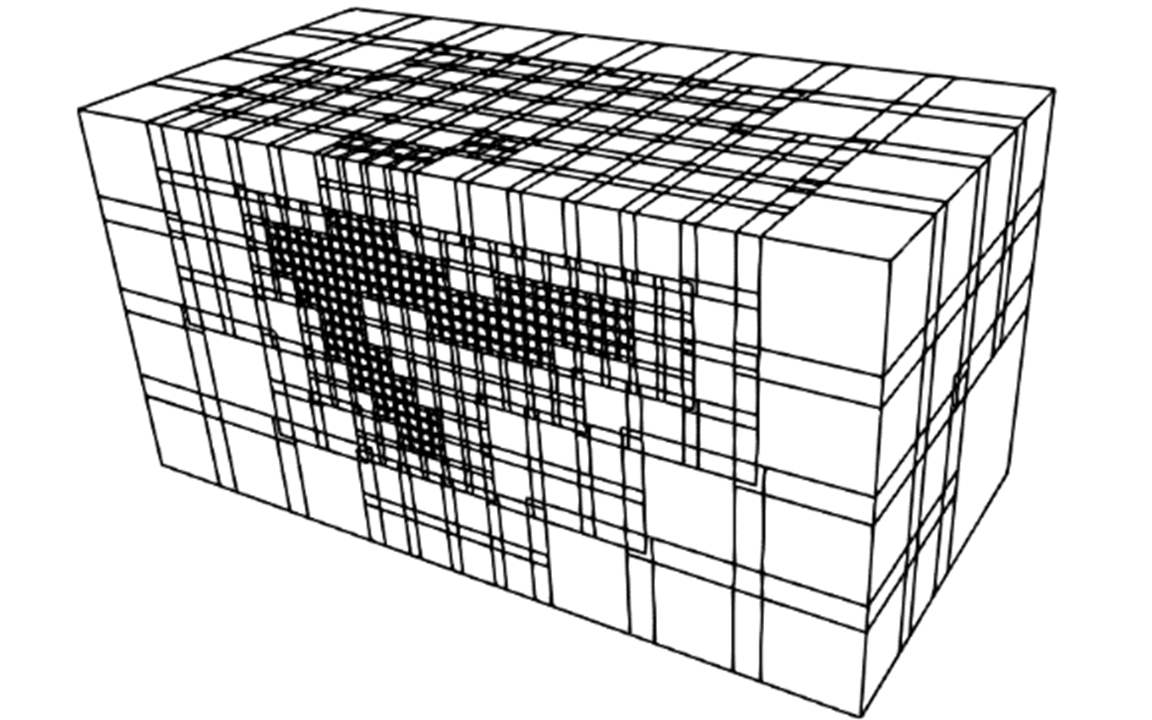
\includegraphics[width=2in]{projects/2.3.4-DataViz/2.3.4.13-ECP-VTK-m/VTKm-Multiblock}\quad
  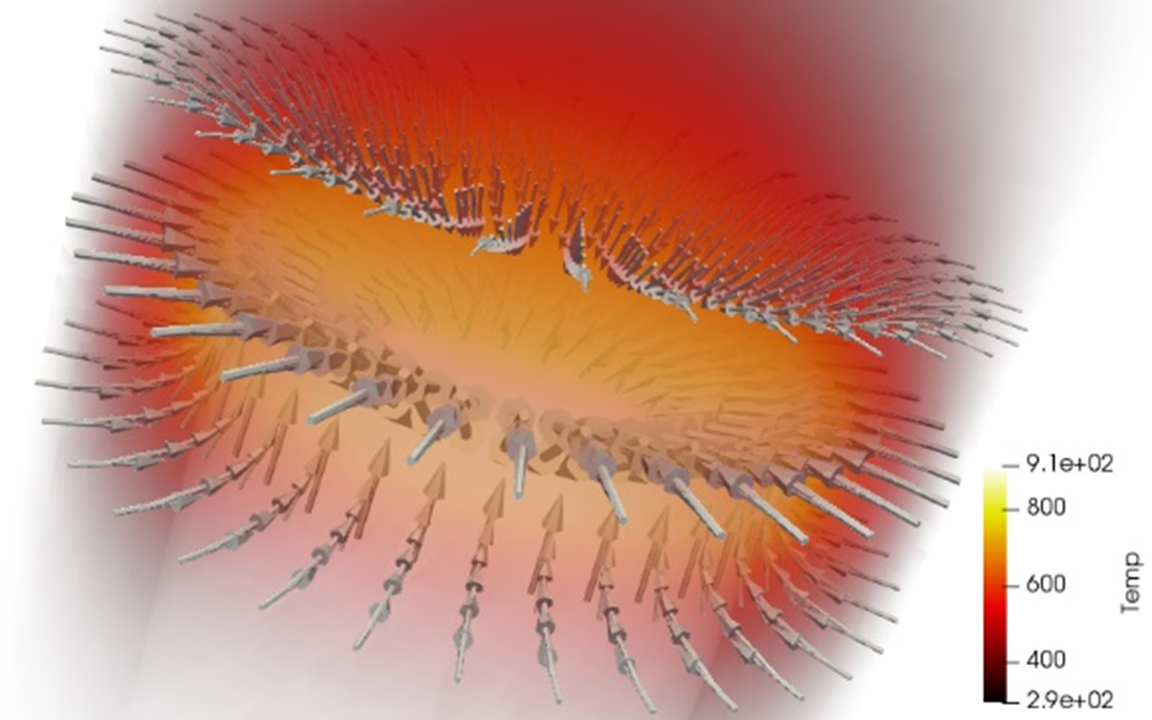
\includegraphics[width=2in]{projects/2.3.4-DataViz/2.3.4.13-ECP-VTK-m/VTKm-Gradients}\quad
  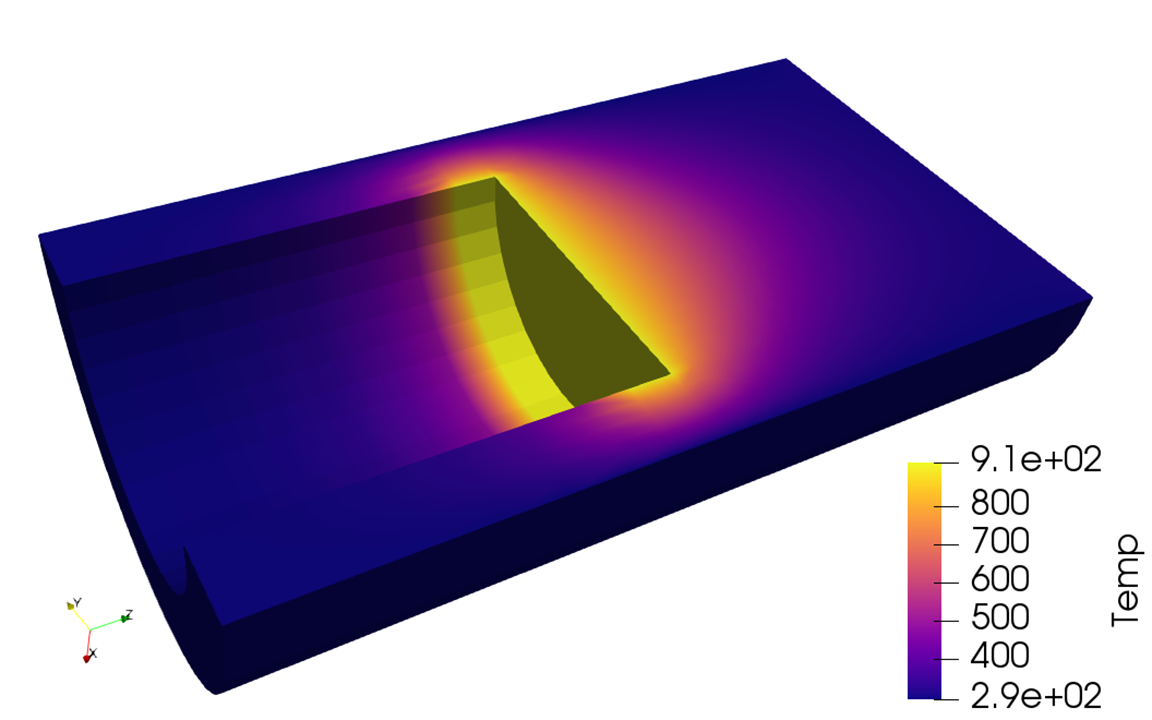
\includegraphics[width=2in]{projects/2.3.4-DataViz/2.3.4.13-ECP-VTK-m/VTKm-FieldToColors}
  \caption{
    Examples of recent progress in VTK-m include (from left to right) multiblock data structures, gradient estimation, and mapping of fields to colors.
  }
  \label{fig:VTKmRecent}
\end{figure}

\paragraph{Recent Progress}
The VTK-m project is organized into many implementation activities.
The following features have been completed in the FY18 fiscal year.

\begin{itemize}
\item \textbf{Multiblock Data:}
  Treat multiple blocks of data, such as those depicted in Figure \ref{fig:VTKmRecent} at left, as first-class data sets.
  %Direct support of multiblock data not only provides programming convenience but also allows us to improve scheduling tasks for smaller groups of data.
\item \textbf{Gradients:}
  Gradients, depicted in Figure \ref{fig:VTKmRecent} at center, are an important metric of fields and must often be derived using topological data.
  %Gradients are also fundamental in finding important vector field qualities like divergence, vorticity, and q-criterion.
\item \textbf{Field to Colors:}
  Pseudocoloring, demonstrated in Figure \ref{fig:VTKmRecent} at right, is a fundamental feature of scientific visualization, and it depends on a good mechanism of converting field data to colors.
\item \textbf{VTK-m 1.1 Release:}
  VTK-m 1.1 was released in December 2017.
\item \textbf{Extract External Surface:}
  When rendering solid objects, it is only necessary to render the external surface of the object as the interior of the volume is hidden \cite{Lessley2016,Lessley2017}.
  %As such, external surface extraction is one of the most common operations in scientific visualization applications.
\item \textbf{Coordinate system transformations:}
  3D rendering systems operate in Cartesian coordinate systems.
  However, data are sometimes referenced in cylindrical or spherical coordinate systems.% to match the physical structure of the data.
  %Consequently, visualization tools need a fast method to convert coordinates among different spaces.
\item \textbf{Affine Transformations:}
  Affine transformations, which include translate, rotate, and scale, are a common and important method to manipulate objects in 3D space.
\item \textbf{Location Structures:}
  Finding mesh components from a coordinate in space requires search structures.
\item \textbf{Rendering Topological Entities:}
  It is often helpful to analysts to view representations of the constitute components of a mesh.
\item \textbf{OpenMP:}
  %Much of the code we wish to integrate with uses OpenMP \cite{OpenMP}, which can conflict with other threading implementations.
  %VTK-m now supports multiple threading libraries, including OpenMP, to better match the code it integrates with.
  VTK-m now supports OpenMP \cite{OpenMP} to better match the code it integrates with.
\end{itemize}

\paragraph{Next Steps}
Our next efforts include:

\begin{itemize}
\item \textbf{Dynamic Types:}
  %The initial implementation of VTK-m used templating to adjust to different data structures.
  %However, when data types are not known at compile time, which is common in applications like ParaView and VisIt, templating for all possible combinations becomes infeasible.
  Provide mechanisms to enable runtime polymorphism.
\item \textbf{ZFP:}
  We are assisting the ZFP project (WBS 2.3.4.11) by helping them implement {\zfp} in VTK-m and port across ECP platforms.
\item \textbf{Clip:}
  Cuts away a mesh based on a spatial intersection or field values.
\item \textbf{Ghost Cells:}
  Provide better support for ghost/halo regions across blocks in a mesh.
\item \textbf{Merge Points:}
  Combine points in a mesh that can be considered coincident.
\item \textbf{Connected Components:}
  Identify regions in a mesh where all cells are topologically connected to each other.
\item \textbf{Particle Advection:}
  Many flow visualization algorithms depend on computing the movement of weightless particles in a flow vector field.
%% \item \textbf{Lightweight Cell Library:}
%%   There is much repetition between VTK-m and other visualization code to perform operations on cells.
%%   We would like to consolidate that code into a lightweight library.
\end{itemize}

\noindent
{\tiny Sandia National Laboratories is a multimission laboratory managed and operated by National Technology \& Engineering Solutions of Sandia, LLC, a wholly owned subsidiary of Honeywell International Inc., for the U.S. Department of Energy's National Nuclear Security Administration under contract DE-NA0003525. \hfill SAND~2018-13745~R
\par}
